
\chapter{Decaimiento $H^{+}(k)\longrightarrow \bar{U}(p)D(p')$}

Author: Yubián Andrés Bedoya Henao

\section{Descripción del proceso}

Author: Yubián Andrés Bedoya Henao

En este problema consideremos un Higgs cargado que decae a un quark Down y quark Up. Por ser el Higgs un boson, su descripción esta dada por un campo escalar $\phi$, mientras que el par Up-Dawn se describen por medio de campos fermionicos ($\Psi^{U},\Psi^{D}$).
Denotamos la masa del Higgs $H^{+}$ por $m_H$ y la masa del par de quarks por $m_d$ para el quark Down y $m_u$ para el quark Up. Se supone que $m_H > m_u + m_d$, con el proposito de que cinematicamente sea posible tener el decaimiento de la particula $H^{+}$ al par de quarks Up-Down.
Este proceso se puede denotar por :
\[
 H^{+}(k)\longrightarrow \bar{U}(p)D(p')
\]

donde $k,p,p'$ son los cuadrimomentos de las particulas. El objetivo es calcular los elementos de la matriz $S$ y la amplitud de caimiento $\Gamma$ para este proceso.
En la figura 1 se muestra un diagrama de Feynman del proceso en estudio.

\section{Lagrangiano}
El decaimiento de este proceso se da via una interaccion Yukawa donde el termino mas relevante es:
\begin{equation}
 \mathcal{L}=\bar{U}[K \rho^{D} P_R- \rho^{U} K P_L]D H^{+}
\end{equation}
donde $\rho^{U}=\frac{\sqrt{2}m_u\cot\beta}{v}$, $\rho^{D}=\frac{-\sqrt{2}m_d\tan\beta}{v}$, $P_{R,L}=\frac{1}{2}(1\pm\gamma^{5})$ y $K$ es la matriz de Cabibbo-Kobayashi-Maskawa que en nuestro caso la tomamos como la matriz identidad.
\section{matriz-S}
\begin{figure}
\begin{center}
 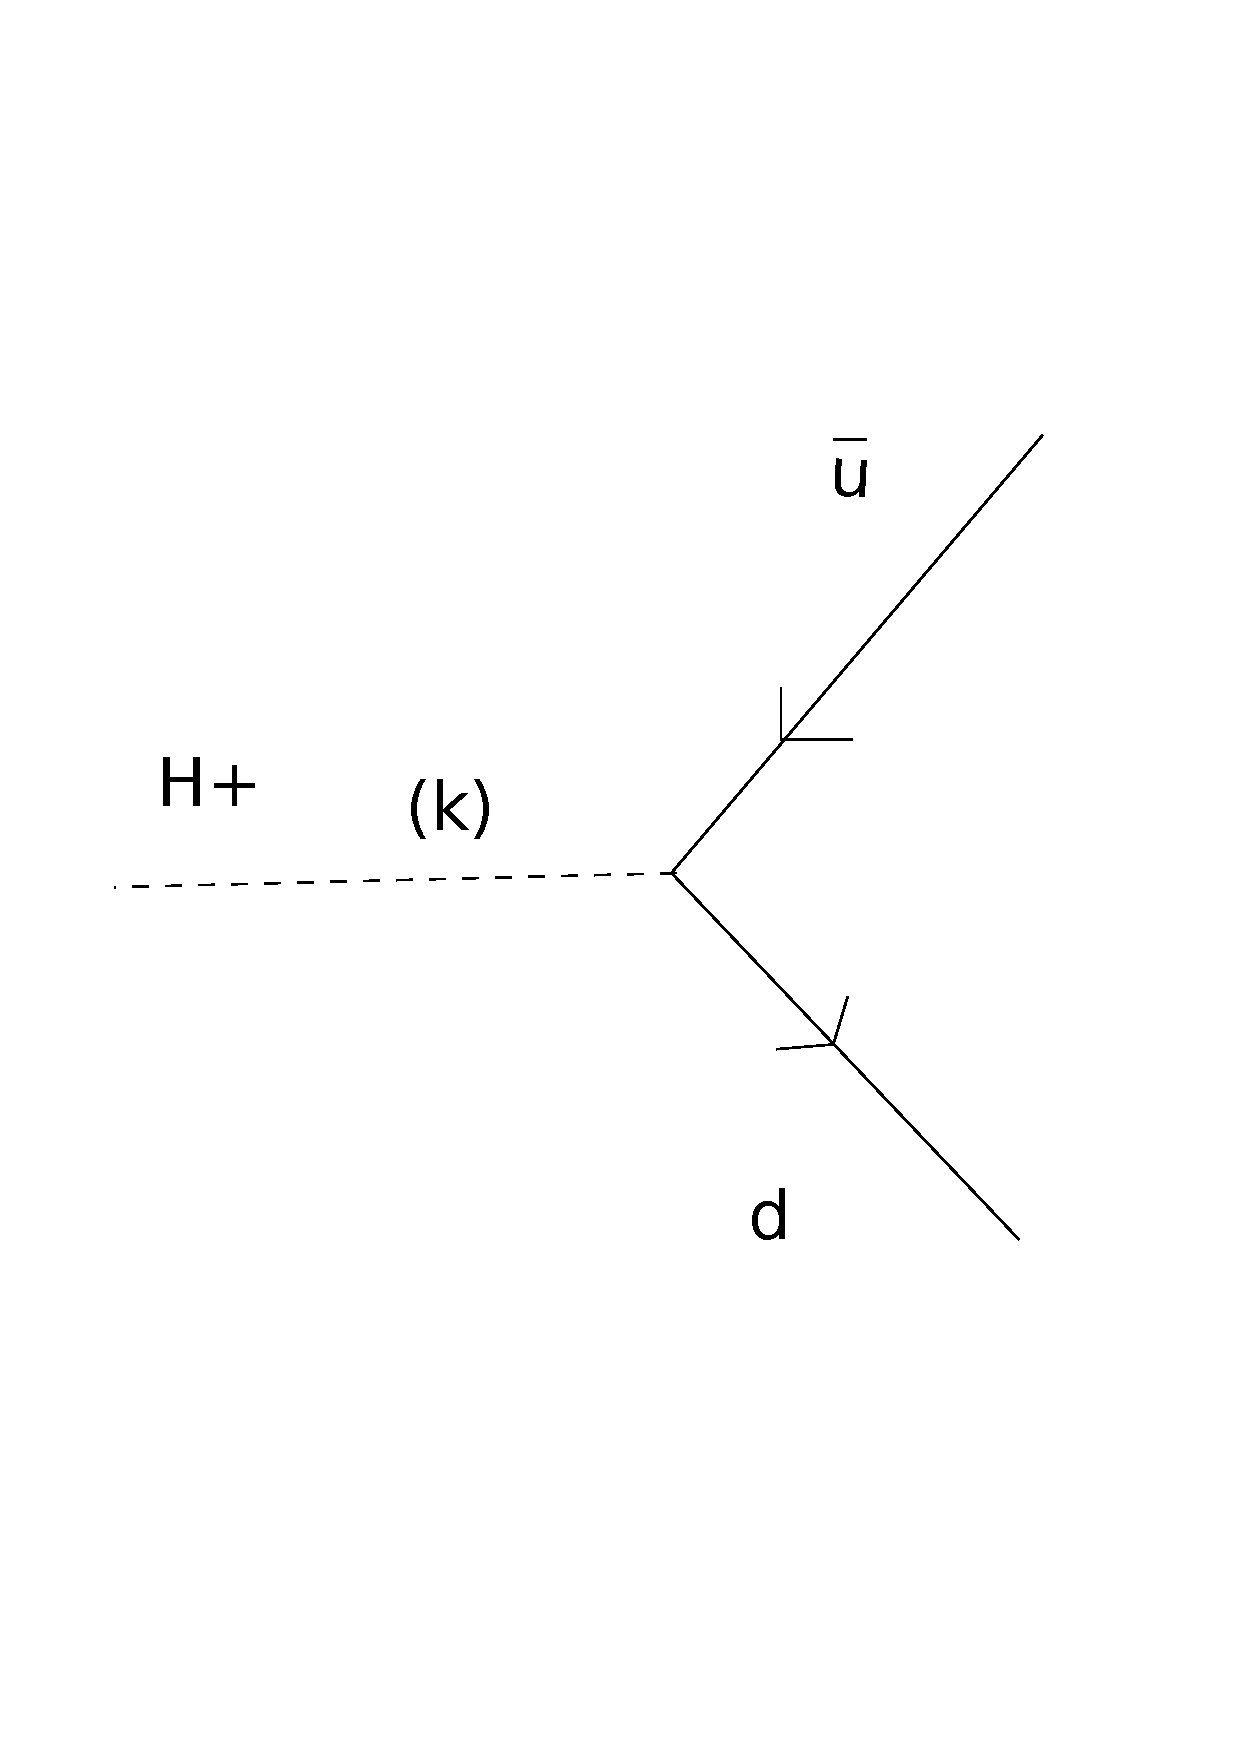
\includegraphics[width=0.5\textwidth]{./ProcesoYubian.pdf}
 \caption{Diagrama de Feynman del proceso}
\end{center}
\end{figure}
El Hamiltoniano de interaccion deriva del lagrangiano de la manera usual. Para la interaccion fermion-escalar se tiene
\begin{equation}
  \mathcal{H}_I=-:\mathcal{L}:
=-:\bar{\Psi}^{U}M\Psi^{D}\phi:
\end{equation}
con $M$ definida como $M= \rho^{D} P_R- \rho^{U} P_L=c_1+c_2\gamma^{5}$ y $c_1=\frac{1}{2}(\rho^{D} - \rho^{U})$, $c_1=\frac{1}{2}(\rho^{D} + \rho^{U})$
Ahora miremos el termino lineal en el  Hamiltoniano de interaccion en la matriz $S$
\[
 S^{(1)}=-i \int d^4x \mathcal{H}_I\\
\]
\[
 =-i \int d^4x :\bar{\Psi}^{U}M\Psi^{D}\phi:
\]
\[
 =-i \int d^4x :(\bar{\Psi}^{U}_{+}+\bar{\Psi}^{U}_{-})M(\Psi^{D}_{+}+\Psi^{D}_{-})(\phi_{+}+\phi_{-}):
\]
Donde el único término que contribuye al elemento de matriz en el proceso viene dado por:
\[
 S^{(1)}=i \int d^4x :\bar{\Psi}^{U}_{-}M\Psi^{D}_{-}\phi_{+}:
\]
El elemento de matriz de este término entre el estado inicial y el estado final es
\[
 S^{(1)}_{fi}=i \int d^4x \langle U(p)\bar{D}(p')|\bar{\Psi}^{D}_{-}\Psi^{D}_{-}\phi_{+}|H^{+}(k)\rangle
\]
Donde se define el estado de una paricula como
\begin{equation}
 |H^{+}(k)\rangle=\sqrt{\frac{1}{V}}a^{\dagger}(k)|0\rangle
\end{equation}
Y de manera similar se tiene
\begin{equation}
 |U(p,s)\rangle=\sqrt{\frac{1}{V}}a^{\dagger}_s(p)|0\rangle
\end{equation}
\begin{equation}
 |\bar{D}(p,s)\rangle=\sqrt{\frac{1}{V}}b^{\dagger}_s(p')|0\rangle
\end{equation}
Ahora podemos escribir la acción de los operadores de campo sobre los diferentes estados de la partícula
usando la descomposición de Fourier del campo escalar y teniendo en que $a_p|o\rangle=0$
\[
 \phi_{+}|H^{+}(k)\rangle=\int d^3p \frac{1}{(2\pi)^3\sqrt{2\omega_p}}\hat{a}_p e^{-ip.x}|H^{+}(k)\rangle
\]
\[
 =\int d^3p \frac{1}{(2\pi)^3\sqrt{2\omega_p}}\hat{a}_p e^{-ip.x}\sqrt{\frac{1}{V}}\hat{a}^{\dagger}(k)|0\rangle
\]
\[
 =\int d^3p \frac{1}{(2\pi)^3\sqrt{2\omega_p V}} e^{-ip.x}[\hat{a}_p,\hat{a}^{\dagger}_k]|0\rangle
\]
\[
 =\int d^3p \frac{\delta^3(\mathbf{p}-\mathbf{k})}{(2\pi)^3\sqrt{2\omega_p V}} e^{-ip.x}|0\rangle
\]
\[
 =\frac{1}{(2\pi)^3\sqrt{2\omega_k V}}e^{-ik.x}|0\rangle
\]
De manera similar, se tiene:
\[
 \Psi_{+}^{U}(x)|U(p)\rangle=\frac{1}{(2\pi)^3\sqrt{2E_p V}}u(\mathbf{p})e^{-ip.x}|0\rangle
\]
\[
 \bar{\Psi}_{+}^{D}(x)|\bar{D}(p')\rangle=\frac{1}{(2\pi)^3\sqrt{2E_{p'} V}}\bar{v}(\mathbf{p'})e^{-ip'.x}|0\rangle
\]
Donde $\omega_k$ y $E_p$ representan la energía para los campos escalar y fermiónico respectivamente. Tomando el adjunto de 
los operadores anteriores nos queda:
\[
\langle H^{+}(k)|\phi_{-}(x)=\langle 0|\frac{1}{(2\pi)^3\sqrt{2\omega_k V}}e^{ik.x}
\]
\[
 \langle U(p)|\bar{\Psi}_{-}^{U}(x)=\langle 0|\frac{1}{(2\pi)^3\sqrt{2E_p V}}\bar{u}(\mathbf{p})e^{ip.x}
\]
\[
 \langle\bar{D}(p')|\Psi_{-}^{D}(x)=\langle 0 |\frac{1}{(2\pi)^3\sqrt{2E_{p'} V}}v(\mathbf{p'})e^{ip'.x}
\]
Así nos queda que el elemento de matriz de primer orden entre los estados inicial y final es:
\[
 S^{(1)}_{fi}=i \int d^4x e^{i(p+p'-k).x}\frac{\bar{u}_s(\mathbf{p})M v_{s'}(\mathbf{p'})}{\sqrt{2\omega_k V}\sqrt{2E_p V}\sqrt{2E_{p'} V}}
\]
\begin{equation}
=\left[\frac{1}{\sqrt{2\omega_k V}}\frac{1}{\sqrt{2E_p V}}\frac{1}{\sqrt{2E_{p'}V}} \right](2\pi)^4 \delta^4(k-p-p')[i\bar{u}_s (\mathbf{p})Mv_{s'} (\mathbf{p'})]
\end{equation}


\section{Cálculo del proceso}
De la expresión anterior de $S^{(1)}_{fi}$ se tiene que
\begin{equation}
 i\mathcal{M}_{fi}=i\bar{u}_s(\mathbf{p})M v_{s'}(\mathbf{p'})
\end{equation}
Ahora teniendo en cuenta que $M= \rho^{D} P_R- \rho^{U} P_L=c_1+c_2\gamma^{5}$ nos queda
\[
 \mathcal{M}_{fi}=\bar{u}(s_1,p_1) [c_1+c_2\gamma^{5}] v(s_2,p_2)
\]
\[
 =\bar{u}(s_1,p_1) c_1v(s_2,p_2)+\bar{u}(s_1,p_1)c_2\gamma^{5}v(s_2,p_2)
\]
\[
  =c_1\bar{u}(s_1,p_1)v(s_2,p_2)+ c_2\bar{u}(s_1,p_1) \gamma^{5}v(s_2,p_2)
\]
tomando el hermítico conjugado de esta expresión obtenemos
\[
 \mathcal{M}_{fi}^{\dagger}=c_1[\bar{u}(s_1,p_1) v(s_2,p_2)]^{\dagger}+ c_2[\bar{u}(s_1,p_1) \gamma^{5} v(s_2,p_2)]^{\dagger}
\]
\[
 =c_1[v^{\dagger}(s_2,p_2)\bar{u}^{\dagger}(s_1,p_1)]+ c_2[v^{\dagger}(s_2,p_2) \gamma^{5}\bar{u}^{\dagger}(s_1,p_1)]
\]
\[
 =c_1[v^{\dagger}(s_2,p_2)(u^{\dagger}(s_1,p_1)\gamma^{0})^{\dagger}]+ c_2[v^{\dagger}(s_2,p_2) \gamma^{5}(u^{\dagger}(s_1,p_1)\gamma^{0})^{\dagger}]
\]
\[
 =c_1[v^{\dagger}(s_2,p_2)(\gamma^{0})^{\dagger}u(s_1,p_1)]+ c_2[v^{\dagger}(s_2,p_2) \gamma^{5}(\gamma^{0})^{\dagger}u(s_1,p_1))]
\]
\[
 =c_1[v^{\dagger}(s_2,p_2)\gamma^{0}u(s_1,p_1)]+ c_2[v^{\dagger}(s_2,p_2) \gamma^{5}\gamma^{0}u(s_1,p_1))]
\]
\[
 =c_1[\bar{v}(s_2,p_2)u(s_1,p_1)]- c_2[\bar{v}(s_2,p_2) \gamma^{5}u(s_1,p_1))]
\]
asi
\[
 |\mathcal{M}_{fi}|^{2}=\mathcal{M}_{fi}\mathcal{M}_{fi}^{\dagger}
\]
\[
 =c_1^{2}\bar{u}(s_1,p_1)v(s_2,p_2)\bar{v}(s_2,p_2)u(s_1,p_1)-c_1c_2\bar{u}(s_1,p_1)v(s_2,p_2)\bar{v}(s_2,p_2) \gamma^{5}u(s_1,p_1)
\]
\[
+c_2c_1\bar{u}(s_1,p_1) \gamma^{5}v(s_2,p_2)\bar{v}(s_2,p_2)u(s_1,p_1)-c_2^{2}\bar{u}(s_1,p_1) \gamma^{5}v(s_2,p_2)\bar{v}(s_2,p_2) \gamma^{5}u(s_1,p_1)
\]
sumando sobre las proyecciones de espin de las particulas finales obtenemos
\[
 \sum_{s_1s_2}|\mathcal{M}_{fi}|^{2}=c_1^{2}\sum_{s_1s_2}^{(1)}-c_1c_2\sum_{s_1s_2}^{(2)}+c_2c_1\sum_{s_1s_2}^{(3)}-c_2^{2}\sum_{s_1s_2}^{(4)}
\]
donde:
\[
 \sum_{s_1s_2}^{(1)}=\sum_{s_1s_2}(\bar{u}(s_1,p_1)v(s_2,p_2))(\bar{v}(s_2,p_2)u(s_1,p_1))
\]
\[
 =\sum_{s_1s_2}(\bar{u}_{\alpha}(s_1,p_1)v_{\alpha}(s_2,p_2))(\bar{v}_{\beta}(s_2,p_2)u_{\beta}(s_1,p_1))
\]
\[
  =\sum_{s_1s_2}(u_{\beta}(s_1,p_1)\bar{u}_{\alpha}(s_1,p_1))(v_{\alpha}(s_2,p_2)\bar{v}_{\beta}(s_2,p_2))
\]
\[
 =\sum_{s_1}(u_{\beta}(s_1,p_1)\bar{u}_{\alpha}(s_1,p_1))\sum_{s_2}(v_{\alpha}(s_2,p_2)\bar{v}_{\beta}(s_2,p_2)) 
\]
\[
 =(\not p_1+m_1)_{\beta\alpha}(\not p_2-m_2)_{\alpha\beta}
\]
\[
 =Tr[(\not p_1+m_1)(\not p_2-m_2)]
\]
teniendo en cuenta que $Tr[\gamma_{\nu}]=0$ y las relaciones de conmutación de las matrices $\gamma_{\mu}$,obtenemos
\[
 Tr[\gamma_{\mu}\gamma_{\nu}]=Tr[-\gamma_{\nu}\gamma_{\mu}+2g^{\mu\nu}]=Tr[-\gamma_{\nu}\gamma_{\mu}]+2g^{\mu\nu}Tr[I]
\]
\[
 =-Tr[\gamma_{\mu}\gamma_{nu}]+2g^{\mu\nu}4
\]
\[
 \Rightarrow Tr[\gamma_{\mu}\gamma_{\nu}]=4g^{\mu\nu}
\]
De esta manera
\[
 Tr[(\not p_1+m_1)(\not p_2-m_2)]=Tr[(\gamma_{\mu}p^{\mu}_1+m_1)(\gamma_{\nu}p^{\nu}_2-m_2)]
\]
\[
 =Tr[\gamma_{\mu}\gamma_{\nu}p^{\mu}_1p^{\nu}_2-m_2\gamma_{\mu}p^{\mu}_1+m_1\gamma_{\nu}p^{\nu}_2-m_1m_2]
\]
\[
 =p^{\mu}_1p^{\nu}_2Tr[\gamma_{\mu}\gamma_{\nu}]-4m_1m_2
\]
\[
 =4g_{\mu\nu}p^{\mu}_1p^{\nu}_2-4m_1m_2=4(p_1.p_2-m_1m_2)
\]
\[
 \Rightarrow  \sum_{s_1s_2}^{(1)}=4(p_1.p_2-m_1m_2)
\]
pero $M=E_1+E_2$ y $|\mathbf{p_1}|=|\mathbf{p_2}|$ entonces $E_1E_2=\frac{M^{2}-E^{2}_1-E^{2}_2}{2}$ por tanto
\[
 p_1.p_2-m_1m_2=E_1E_2-\mathbf{p_1}.\mathbf{p_2}-m_1m_2
\]
\[
 =E_1E_2+\mathbf{p_1}^{2}-m_1m_2
\]
\[
 =frac{M^{2}-E^{2}_1-E^{2}_2}{2}+\mathbf{p_1}^{2}-m_1m_2
\]
\[
 =\frac{M^{2}-m^{2}_1-\mathbf{p_1}^{2}-m^{2}_2-\mathbf{p_1}^{2}}{2}+\mathbf{p_1}^{1}-m_1m_2
\]
\[
 =\frac{M^{2}-m^{2}_1-m^{2}_2-2m_1m_2}{2}
\]
\[
 =\frac{M^{2}-(m_1+m_2)^{2}}{2}
\]
finalmente se tiene que
\[
 \sum_{s_1s_2}^{(1)}=2[M^{2}-(m_1+m_2)^{2}]
\]
Ahora hallemos el valor de $\sum_{s_1s_2}^{(2)}$ la cual esta dada por
\[
 \sum_{s_1s_2}^{(2)}=\sum_{s_1s_2}\bar{u}(s_1,p_1)v(s_2,p_2)\bar{v}(s_2,p_2) \gamma^{5}u(s_1,p_1)
\]
\[
 =\sum_{s_1s_2}(\bar{u}_{\alpha}(s_1,p_1)v_{\alpha}(s_2,p_2))(\bar{v}_{\sigma}(s_2,p_2) \gamma^{5}_{\beta\sigma}u_{\sigma}(s_1,p_1))
\]
\[
 =\sum_{s_1s_2}(v_{\alpha}(s_2,p_2)(\bar{v}_{\sigma}(s_2,p_2)) \gamma^{5}_{\beta\sigma}(u_{\sigma}(s_1,p_1)\bar{u}_{\alpha}(s_1,p_1))
\]
\[
 =\sum_{s_2}(v_{\alpha}(s_2,p_2)(\bar{v}_{\sigma}(s_2,p_2)) \gamma^{5}_{\beta\sigma}\sum_{s_1}(u_{\sigma}(s_1,p_1)\bar{u}_{\alpha}(s_1,p_1))
\]
\[
 =(\not p_2-m_2)_{\alpha\beta}\gamma^{5}_{\beta\sigma}(\not p_1+m_1)_{\sigma\alpha}
\]
\[
 =Tr[(\not p_2-m_2)\gamma^{5}(\not p_1+m_1)]
\]
\[
 =Tr[(\gamma_{\mu}p^{\mu}_2-m_2)\gamma^{5}(\gamma_{\nu}p^{\nu}_1+m_1)]
\]
\[
 =p^{\mu}_2p^{\nu}_1Tr[\gamma_{\mu}\gamma^{5}\gamma_{\nu}]+m_1p^{\mu}_2Tr[\gamma_{\mu}\gamma^{5}]-m_2p^{\nu}_1Tr[\gamma^{5}\gamma_{\nu}]-m_1m_2Tr[\gamma^{5}]
\]
\[
 =0
\]
ya que $Tr[\gamma_{\mu}\gamma^{5}\gamma_{\nu}]=0$, $Tr[\gamma_{\mu}\gamma^{5}]=0$ y $Tr[\gamma^{5}]=0$ como es facil de demostrar.
de manera similar se prueba que $\sum_{s_1s_2}^{(3)}=0$. Finalmente calculemos $\sum_{s_1s_2}^{(4)}$, donde teniendo en cuenta que $Tr[\gamma^{5}]=0$, $Tr[\gamma_{\mu}]=0$ y que $(\gamma^{5})^{2}=1$ y $\gamma_{\mu}\gamma^{5}=-\gamma^{5}\gamma_{\mu}$ encontramos
\[
 \sum_{s_1s_2}^{(4)}=\sum_{s_1s_2}\bar{u}(s_1,p_1)\gamma^{5}v(s_2,p_2)\bar{v}(s_2,p_2) \gamma^{5}u(s_1,p_1)
\]
\[
 =\sum_{s_1s_2}(\bar{u}_{\alpha}(s_1,p_1)\gamma^{5}_{\alpha\beta}v_{\beta}(s_2,p_2))(\bar{v}_{\sigma}(s_2,p_2) \gamma^{5}_{\sigma\lambda}u_{\lambda}(s_1,p_1))
\]
\[
 =\sum_{s_1}(u_{\lambda}(s_1,p_1)\bar{u}_{\alpha}(s_1,p_1))\gamma^{5}_{\alpha\beta}\sum_{s_2}(v_{\beta}(s_2,p_2)\bar{v}_{\sigma}(s_2,p_2)) \gamma^{5}_{\sigma\lambda}
\]
\[
 =(\not p_1+m_1)_{\lambda\alpha}\gamma^{5}_{\alpha \beta}(\not p_2-m_2)_{\beta\sigma}\gamma^{5}_{\sigma\lambda}
\]
\[
 =Tr[(\not p_1+m_1)\gamma^{5}(\not p_2-m_2)\gamma^{5}]
\]
\[
 =Tr[(\gamma_{\mu}p^{\mu}_1+m_1)\gamma^{5}(\gamma_{\nu}p^{\nu}_2-m_2)\gamma^{5}]
\]
\[
 =Tr[p^{\mu}_1p^{\nu}_2\gamma_{\mu}\gamma^{5}\gamma_{\nu}\gamma^{5}-m_2p^{\mu}_1\gamma_{\mu}\gamma^{5}\gamma^{5}
+m_1p^{\nu}_2\gamma^{5}\gamma_{\nu}\gamma^{5}-m_1m_2\gamma^{5}\gamma^{5}]
\]
\[
 =-p^{\mu}_1p^{\nu}_2Tr[\gamma_{\mu}\gamma_{\nu}]-4m_1m_2
\]
\[
 =-p^{\mu}_1p^{\nu}_2(4g_{\mu\nu})-4m_1m_2
\]
\[
 =-4(p_1.p_2+m_1m_2)
\]
donde
\[
 p_1.p_2+m_1m_2=E_1E_2-\mathbf{p_1}.\mathbf{p_2}+m_1m_2
\]
\[
 =E_1E_2+\mathbf{p_1}^{2}+m_1m_2
\]
\[
 =frac{M^{2}-E^{2}_1-E^{2}_2}{2}+\mathbf{p_1}^{2}+m_1m_2
\]
\[
 =\frac{M^{2}-m^{2}_1-\mathbf{p_1}^{2}-m^{2}_2-\mathbf{p_1}^{2}}{2}+\mathbf{p_1}^{1}+m_1m_2
\]
\[
 =\frac{M^{2}-m^{2}_1-m^{2}_2+2m_1m_2}{2}
\]
\[
 =\frac{M^{2}-(m_1-m_2)^{2}}{2}
\]
\[
 \Rightarrow \sum_{s_1s_2}^{(4)}=-2[M^{2}-(m_1-m_2)^{2}]
\]
Asi tenemos finalmente 
\begin{equation}
 \sum_{s_1s_2}|\mathcal{M}_{fi}|^{2}=2c_1^{2}[M^{2}-(m_1+m_2)^{2}]+2c_2^{2}[M^{2}-(m_1-m_2)^{2}]
\end{equation}
por tanto la tasa de decaimiento de este proceso es 
\begin{equation}
 \Gamma=\frac{1}{2M}\int\frac{d^3p_1}{(2\pi)^32E_1}\int\frac{d^3p_2}{(2\pi)^32E_2}(2\pi)^4\delta(k-p_1-p_2)\sum_{s_1s_2}|\mathcal{M}_{fi}|^2
\end{equation}
Reemplazando $(8)$ en $(9)$ yluego integrando llegamos a 
\begin{equation}
 \Gamma=\frac{Mc_1^{2}}{8\pi}\left(1-\frac{4m_1m_2}{M^2}\right)^{3/2}+\frac{Mc_2^{2}}{8\pi}\left(1+\frac{4m_1m_2}{M^2}\right)^{3/2}
\end{equation}
Reemplazando $M=m_H=115 GeV$, $m_1=m_u=1,7 MeV$, $m_2=m_d=4,1 MeV$,$v=246 GeV$ y recordando las expresiones de $c_1$ y $c_2$ con $\tan\beta=10$ se obtiene
\begin{equation}
 \Gamma=127,105 eV
\end{equation}
 y 
\begin{equation}
 \tau=\frac{1}{\Gamma}=3,254\times 10^{-17} s
\end{equation}

\section{CalcHEP comparison}
No se pudo realizar el cálculo en CalcHEP debido a que el paquete correspondiente a este proceso contenía errores.



\section{Copyright}

\includegraphics[scale=0.5]{cc} Creative Commons Attribution-Share Alike 3.0 United States License.


%%% Local Variables: 
%%% mode: latex
%%% TeX-master: "qft_samples"
%%% End: 
